\apendice{Especificación de Requisitos}

\section{Introducción}

En esta sección se presentarán los requisitos y casos de uso que han dado lugar a la funcionalidad de la aplicación. Esta información irá acompañada del modelo relacional y de los diagramas entidad relación.

\section{Objetivos generales}

Los principales objetivos del proyecto son: 

\begin{itemize}
	
	\item Dar soporte a través de una aplicación web a los resultados obtenidos tras la ejecución del algoritmo de optimización que posee el cliente.
	
	\item Lograr una aplicación intuitiva sin problemas de usabilidad para el usuario.

	\item Crear una administración que permita crear, editar y eliminar cualquiera de las entidades mediante formularios.
	
	\item Para las entidades con registros en instantes de tiempo, dar posibilidad al usuario de subir una hoja de cálculo para actualizar los datos.
	
	\item Innovar en como el tribunal de proyectos puede hacer una batería de pruebas sobre una aplicación fuertemente basada en una interfaz de usuario. Para ello se implementará un botón de restauración de la base de datos.
	
	\item Construir una pantalla desde la que el cliente pueda ejecutar el algoritmo.

\end{itemize}

\section{Catalogo de requisitos}

Los requisitos que debe satisfacer la aplicación son:

\subsection{Requisitos funcionales}

\begin{itemize}
	
	\item \textbf{RF-1:} Administrar mediante formularios las entidades correspondientes a: 

		\begin{itemize}
			
			\item Arcos entre dos regiones.
			\item Tipo de conexión de ese arco.
			\item Relación entre el arco y el tipo de arco.
			\item Países.
			\item Combustibles.
			\item Tecnologías
			\item Regiones.
			\item Relación entre combustibles y tecnologías.
			\item Relación entre regiones y tecnologías.
			
		\end{itemize}
	
	\item \textbf{RF-2:} Administración para las entidades correspondientes a través de una hoja de cálculo en la que se guarda un valor concreto para cada una de las horas del año en una región determinada:
	
		\begin{itemize}
			
			\item Datos acerca del clima.
			\item Datos acerca de fuentes renovables.
			\item Datos de demanda.
			
		\end{itemize}
	
	\item \textbf{RF-3:} El usuario de la aplicación podrá tener acceso a la visualización de cada una de las entidades. Se realizará a través de tablas paginadas con posibilidad de acceder a un detalle más exhaustivo pulsando en cada elemento.
	
	\item \textbf{RF-4:} El usuario podrá exportar una hoja de cálculo con los datos de las entidades cuya administración funciona con la subida de un fichero. Esta misma hoja de cálculo, podrá modificarla y subirla para actualizar los datos.
	
	\item \textbf{RF-5:} El usuario tras realizar pruebas de funcionalidad sobre la aplicación, podrá restablecer la base de datos a un punto de partida pulsando un botón situado en la cabecera.
	
	\item \textbf{RF-6:} Existirá un control de usuarios en el que haya usuarios con dos posibles roles: administrador y participante.
	
\end{itemize}

\subsection{Requisitos no funcionales}

	\begin{itemize}
	
		\item \textbf{RNF-1:} La aplicación tiene que ser intuitiva y fácil de usar de cara al usuario.
		\item \textbf{RNF-2:} El rendimiento de la aplicación tiene que ser lo más óptimo posible. La navegación entre las diferentes pantallas tiene que ser fluida. 
		\item \textbf{RNF-3:} La aplicación deberá funcionar con normalidad en todos los navegadores.
		
	\end{itemize}
	
\newpage

\section{Especificación de requisitos}

En este apartado se describirán los actores y casos de uso asociados a cada uno de los requisitos definidos anteriormente. 

\subsection{Actores}

Actores presentes en la aplicación:

\begin{itemize}
	\item Administrador de la aplicación: Realiza la primera carga de datos iniciales y prepara la consulta \textit{sql} para poder restablecer la base de datos.
	\item Usuario: Interactúa con la aplicación web.
	\begin{itemize}
		\item Usuario con rol administrador: Tiene acceso al control de usuarios y al botón para restablecer la base de datos.
		\item Usuario con rol participante: Interactúa con la aplicación web sin tener acceso a ninguna funcionalidad especial.
	\end{itemize}
\end{itemize}

\subsection{Diagrama de casos de uso}

\begin{figure}[h]
	\centering
	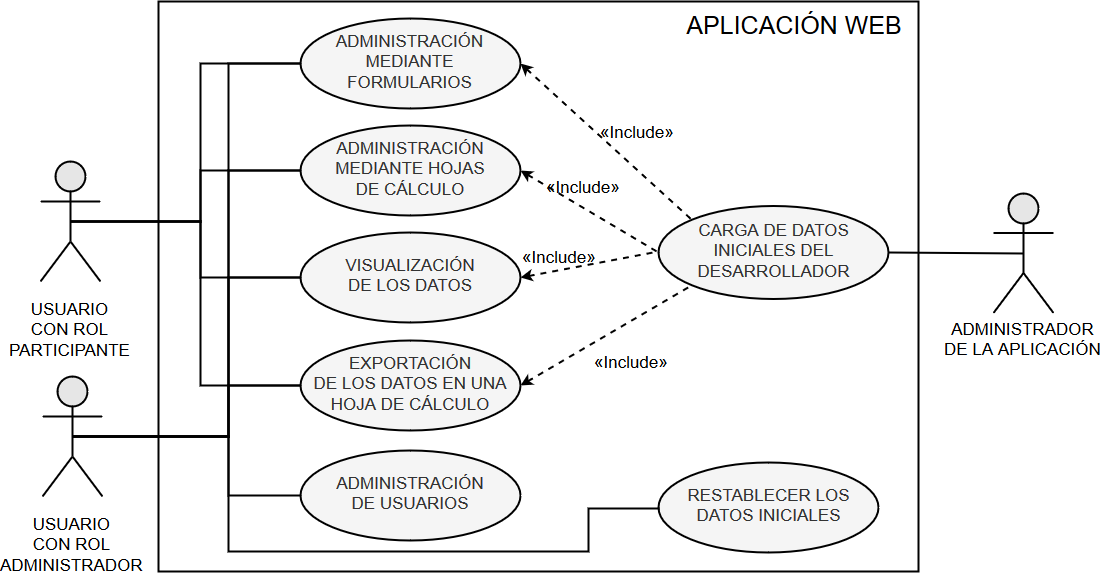
\includegraphics[width=1\textwidth]{/anexos/Requisitos/CasosUso}
	\caption{Diagrama de casos de uso de \textit{Weblectric}.}
	\label{fig:casosUso}
\end{figure}

\begin{figure}[h]
	\centering
	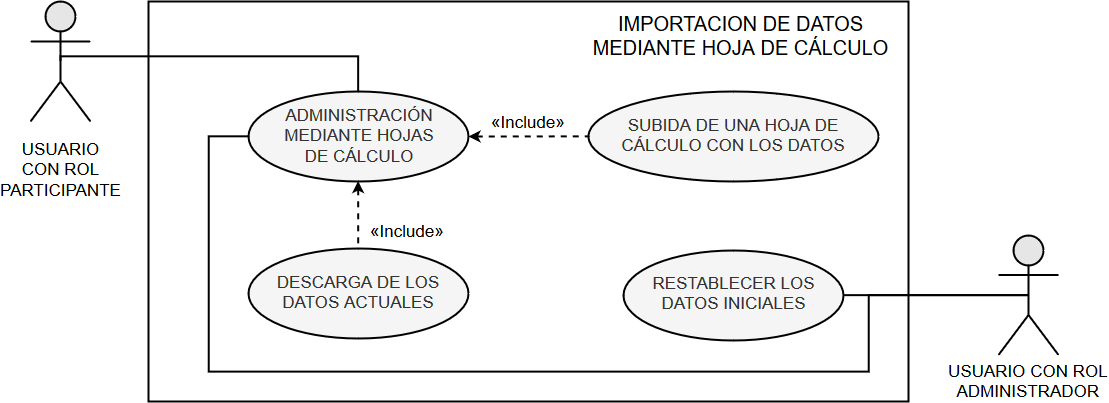
\includegraphics[width=1\textwidth]{/anexos/Requisitos/CasosUsoExcel}
	\caption{Diagrama del casos de uso 2: Administración mediante hojas de cálculo.~\ref{tabla:cu2}.}
	\label{fig:casosUsoExcel}
\end{figure}

\begin{figure}[h]
	\centering
	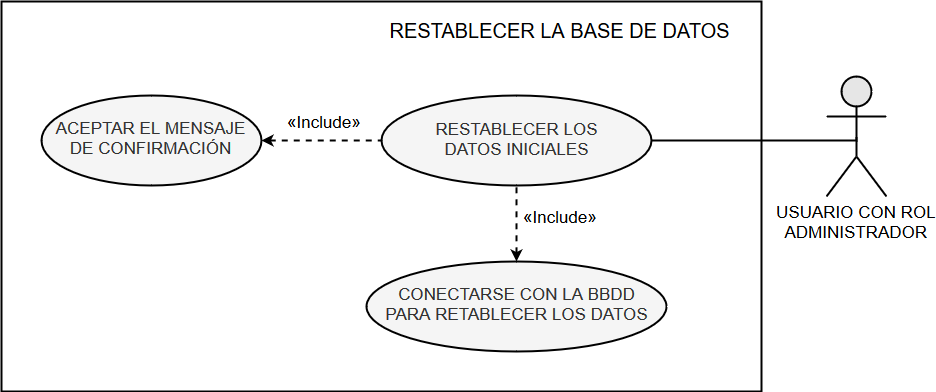
\includegraphics[width=1\textwidth]{/anexos/Requisitos/CasosUsoBBDD}
	\caption{Diagrama del casos de uso 5: Restablecer base de datos.~\ref{tabla:cu5}.}
	\label{fig:CasosUsoBBDD}
\end{figure}

\begin{figure}[h]
	\centering
	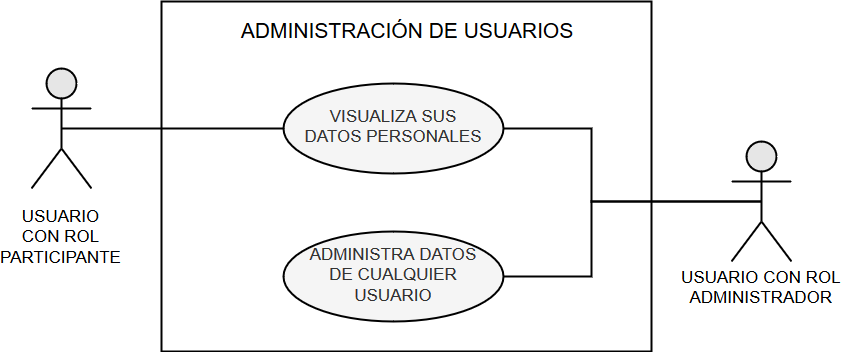
\includegraphics[width=1\textwidth]{/anexos/Requisitos/CasosUsoUsers}
	\caption{Diagrama del casos de uso 6: Administración de usuarios.~\ref{tabla:cu6}.}
	\label{fig:CasosUsoUsers}
\end{figure}

% Caso de uso 1

\begin{table}[h]
	\centering
	\label{tabla:cu1}
	\begin{tabular}{@{}
		>{\columncolor[HTML]{FFFFFF}}p {.25\textwidth} p {.75\textwidth}@{}}
		\toprule
		\textbf{Caso de uso 1}   & \textbf{Administración mediante formularios.} \\ \midrule
		\textbf{Versión}         & 1.0 \\ \midrule
		\textbf{Requisitos}	     & \begin{tabular}[c]{@{}l@{}}
										RF-1
								   \end{tabular} \\ \midrule
		\textbf{Descripción}     & \begin{tabular}[c]{@{}l@{}}
										El usuario podrá crear/editar/borrar elementos de las \\ 
										entidades.
								   \end{tabular} \\ \midrule
		\textbf{Precondiciones}  & \begin{tabular}[c]{@{}l@{}}
										1. Base de datos iniciada.\\ 
										2. Carga inicial de datos realizada.
								   \end{tabular} \\ \midrule
		\textbf{Acciones}        & \begin{tabular}[c]{@{}l@{}}
										En función de la labor que desee realizar, el usuario \\
										interaccionará con los botones de crear/editar/borrar.
								   \end{tabular} \\ \midrule
		\textbf{Postcondiciones} & \begin{tabular}[c]{@{}l@{}}
									    La aplicación emitirá un mensaje de confirmación en caso \\
									    de realizarse una baja y se redireccionará al listado de \\
									    todos los datos y el usuario podrá ver el resultado \\ 
									    de la acción. \\ 
								   \end{tabular} \\ \midrule
		\textbf{Excepciones}     & \begin{tabular}[c]{@{}l@{}}
										1. No haya datos para una entidad.\\ 
										2. Eliminar algún elemento relacionado con otra entidad.
								   \end{tabular} \\ \midrule
		\textbf{Importancia}     & Alta \\ \bottomrule
	\end{tabular}
	\caption{Caso de uso 1 - Administración mediante formularios.}
\end{table}

% Caso de uso 2

\begin{table}[h]
	\centering
	\label{tabla:cu2}
	\begin{tabular}{@{}
			>{\columncolor[HTML]{FFFFFF}}p {.25\textwidth} p {.75\textwidth}@{}}
		\toprule
		\textbf{Caso de uso 2}   &  \textbf{Administración mediante hojas de cálculo.} \\ \midrule
		\textbf{Versión}         &  1.0 \\ \midrule
		\textbf{Requisitos}	     &  \begin{tabular}[c]{@{}l@{}}
										RF-2
									\end{tabular} \\ \midrule
		\textbf{Descripción}     &  \begin{tabular}[c]{@{}l@{}}
										El usuario podrá actualizar los datos subiendo a la \\
										aplicación una hoja de cálculo.
									\end{tabular} \\ \midrule
		\textbf{Precondiciones}  &  \begin{tabular}[c]{@{}l@{}}
										1. Base de datos iniciada.\\ 
										2. Carga inicial de datos realizada.
									\end{tabular} \\ \midrule
		\textbf{Acciones}        &  \begin{tabular}[c]{@{}l@{}}
										1. En usuario deberá entrar en la pantalla \\
										correspondiente a la entidad que quiere modificar. \\
										2. Se deberá descargar la plantilla. \\
										3. Subirá un excel con los datos que desee.
									\end{tabular} \\ \midrule
		\textbf{Postcondiciones} &  \begin{tabular}[c]{@{}l@{}}
										La aplicación se redireccionará al listado de todos los \\ 
										datos y el usuario podrá ver la fecha de la última \\
										subida.
									\end{tabular} \\ \midrule
		\textbf{Excepciones}     &  \begin{tabular}[c]{@{}l@{}}
										Introducir algún elemento extraño en la hoja de cálculo \\
										que agote los recursos de procesado de la máquina \\
										produciendo un error.\\ 
									\end{tabular} \\ \midrule
		\textbf{Importancia}     &  Alta \\ \bottomrule
	\end{tabular}
	\caption{Caso de uso 2 - Administración mediante hojas de cálculo.}
\end{table}

% Caso de uso 3

\begin{table}[h]
	\centering
	\label{tabla:cu3}
	\begin{tabular}{@{}
			>{\columncolor[HTML]{FFFFFF}}p {.25\textwidth} p {.75\textwidth}@{}}
		\toprule
		\textbf{Caso de uso 3}   &  \textbf{Visualización de datos en tablas paginadas.} \\ \midrule
		\textbf{Versión}         &  1.0 \\ \midrule
		\textbf{Requisitos}	     &  \begin{tabular}[c]{@{}l@{}}
										RF-3
									\end{tabular} \\ \midrule
		\textbf{Descripción}     &  \begin{tabular}[c]{@{}l@{}}
										El usuario podrá visualizar un conjunto de datos \\
										en tablas paginadas.
									\end{tabular} \\ \midrule
		\textbf{Precondiciones}  &  \begin{tabular}[c]{@{}l@{}}
										1. Base de datos iniciada.\\ 
										2. Carga inicial de datos realizada. \\
										3. Realización de una consulta.
									\end{tabular} \\ \midrule
		\textbf{Acciones}        &  \begin{tabular}[c]{@{}l@{}}
										1. En usuario deberá de entrar en la pantalla \\
										correspondiente a la entidad que quiere visualizar. \\
										2. Si lo desea, podrá modificar la consulta utilizando \\
										los filtros del buscador. \\
										3. Pulsar el botón de búsqueda para obtener los \\
										nuevos resultados. \\
										4. Si se desea una información más exhaustiva, se podrá \\
										pulsar en el botón de visualización.
									\end{tabular} \\ \midrule
		\textbf{Postcondiciones} &  \begin{tabular}[c]{@{}l@{}}
										Pulsando en el botón de buscar, se actualizará la página \\
										con los nuevos resultados.
									\end{tabular} \\ \midrule
		\textbf{Excepciones}     &  \begin{tabular}[c]{@{}l@{}}
										Introducir filtros que no representen ningún dato.\\ 
									\end{tabular} \\ \midrule
		\textbf{Importancia}     &  Media \\ \bottomrule
	\end{tabular}
	\caption{Caso de uso 3 - Visualización de datos en tablas paginadas.}
\end{table}

% Caso de uso 4

\begin{table}[h]
	\centering
	\label{tabla:cu4}
	\begin{tabular}{@{}
			>{\columncolor[HTML]{FFFFFF}}p {.25\textwidth} p {.75\textwidth}@{}}
		\toprule
		\textbf{Caso de uso 4}   &  \textbf{Exportar datos en hoja de cálculo.} \\ \midrule
		\textbf{Versión}         &  1.0 \\ \midrule
		\textbf{Requisitos}	     &  \begin{tabular}[c]{@{}l@{}}
										RF-4
									\end{tabular} \\ \midrule
		\textbf{Descripción}     &  \begin{tabular}[c]{@{}l@{}}
										El usuario podrá exportar una hoja de cálculo con los \\
										datos de las entidades cuya administración funciona \\
										con la subida de un fichero.
									\end{tabular} \\ \midrule
		\textbf{Precondiciones}  &  \begin{tabular}[c]{@{}l@{}}
			1. Base de datos iniciada.\\ 
			2. Carga inicial de datos realizada. \\
		\end{tabular} \\ \midrule
		\textbf{Acciones}        &  \begin{tabular}[c]{@{}l@{}}
										1. En usuario deberá de entrar en la pantalla \\
										correspondiente a la entidad que quiere exportar. \\
										2. Pulsar sobre el icono exportar.
									\end{tabular} \\ \midrule
		\textbf{Postcondiciones} &  \begin{tabular}[c]{@{}l@{}}
										Se descargará un fichero con los datos actuales \\
										en base de datos.
									\end{tabular} \\ \midrule
		\textbf{Excepciones}     &  \begin{tabular}[c]{@{}l@{}}
										Entidad sin datos cagados. En ese caso los datos \\
										de la exportación estarán vacíos.\\ 
									\end{tabular} \\ \midrule
		\textbf{Importancia}     &  Media \\ \bottomrule
	\end{tabular}
	\caption{Caso de uso 4 - Exportar datos en hoja de cálculo.}
\end{table}

% Caso de uso 6

\begin{table}[h]
	\centering
	\label{tabla:cu6}
	\begin{tabular}{@{}
			>{\columncolor[HTML]{FFFFFF}}p {.25\textwidth} p {.75\textwidth}@{}}
		\toprule
		\textbf{Caso de uso 6}   &  \textbf{Administración de usuarios.} \\ \midrule
		\textbf{Versión}         &  1.0 \\ \midrule
		\textbf{Requisitos}	     &  \begin{tabular}[c]{@{}l@{}}
										RF-6
									\end{tabular} \\ \midrule
		\textbf{Descripción}     &  \begin{tabular}[c]{@{}l@{}}
										Existirá la posibilidad de administrar los usuarios de \\
										la aplicación. Los usuarios con rol administrador \\
										podrán visualizar y modificar los datos de cualquier\\
										usuario mientras que un usuario con rol participante \\
										solo podrá administrar los suyos propios.
									\end{tabular} \\ \midrule
		\textbf{Precondiciones}  &  \begin{tabular}[c]{@{}l@{}}
										 \\
									\end{tabular} \\ \midrule
		\textbf{Acciones}        &  \begin{tabular}[c]{@{}l@{}}
										1. Usuario administrador accede a la pantalla de \\
										usuarios. \\
										2. De los resultados listados en la tabla, elige el usuario \\
										a modificar.\\
										3. Mediante la acción correspondiente, crea, edita \\
										y elimina un usuario.
									\end{tabular} \\ \midrule
		\textbf{Postcondiciones} &  \begin{tabular}[c]{@{}l@{}}
										Redirección a la pantalla principal de los usuarios.
									\end{tabular} \\ \midrule
		\textbf{Excepciones}     &  \begin{tabular}[c]{@{}l@{}}
										Error al ejecutar la acción.\\ 
									\end{tabular} \\ \midrule
		\textbf{Importancia}     &  Media \\ \bottomrule
	\end{tabular}
	\caption{Caso de uso 6 - Administración de usuarios.}
\end{table}